\begin{center}
\begin{tikzpicture}[x=1cm,y=1cm]
%\pgfresetboundingbox
\draw[use as bounding box, anchor = north west,draw,dashed,gray] (-5.5,-3.25) rectangle (5.5,3.25);
\clip (-5.5,-3.25) rectangle (5.5,3.25);
\node[anchor =north west] (text) at (-5.25,3.25){\begin{minipage}{5.0cm}
\visible<1-8>{We have seen that adapting model complexity to fit the problem at hand is generally necessary. However, it is not generally obvious how to do
this is a simple models often lack useful features, e.g. $2^{\textrm{nd}}$ order polynomials have one turning point. Therefore, we need another way 
to prevent over-fitting that is applicable to many different types of model -- \textbf{Regularization}:
}

\begin{align*}
    y(x) &=\sin(2\pi x)
\end{align*}
Note that $f^{*} \notin \mathcal{T}$!\\
\only<2>{Assume $8$ measurements with noise $\mathcal{N}(0,0.2)$}\\
\only<3-4>{Start with degree $2$...\only<4>{What happens when we increase the order?}}
\only<6-8>{\\ What do the risk terms look like?}
\only<8->{\vspace{1.75cm}\\\color{red}{What happens if we add more data?}}
\end{minipage}};
\visible<1>{\node (figure) at (2.75,0){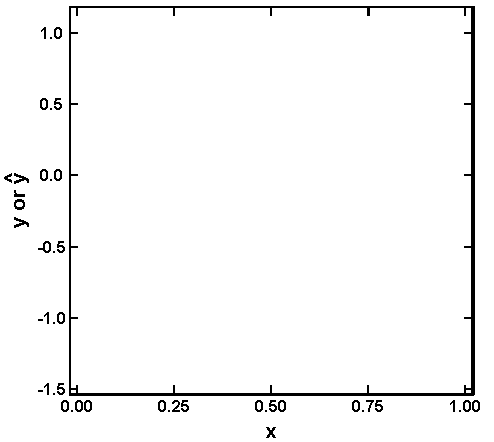
\includegraphics[width=5cm]{satistical_learning/figures/lam_1.pdf}};}
\visible<2>{\node (figure) at (2.75,0){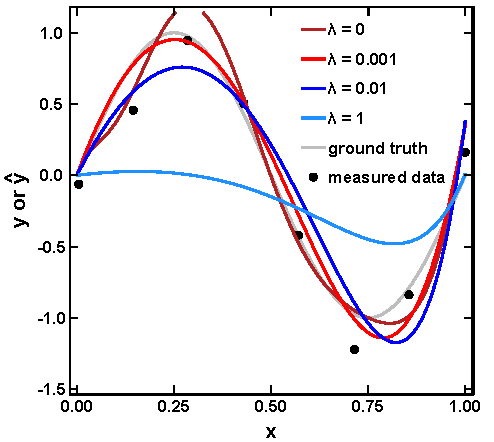
\includegraphics[width=5cm]{satistical_learning/figures/lam_2.pdf}};}
\visible<3>{\node (figure) at (2.75,0){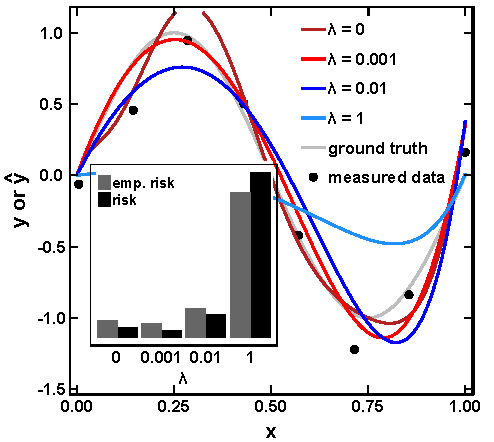
\includegraphics[width=5cm]{satistical_learning/figures/lam_3.pdf}};}
\end{tikzpicture}
\end{center}